\section{Data structure}
\label{sec:data_structure}

\subsection{Description of the data structure}
\label{sec:descriptiondata}
The raw data is \textbf{only} stored in the Via Appia Linux server and there is Python script that needs to be used to generate the converted OSG data, the \textit{createosgdata.py}. The raw data directory is \textit{/home/vadata/DATA/RAW}. OSG data is stored in \textit{/home/vadata/DATA/OSG} and POTREE data is stored in \textit{/home/vadata/DATA/POTREE} (figure \ref{fig:directory_structure_overview}). 

The next subsections explores the RAW data tree in more detail and discusses how to modify and list the data in the RAW data tree.

\begin{figure}[!ht]
 \centering
 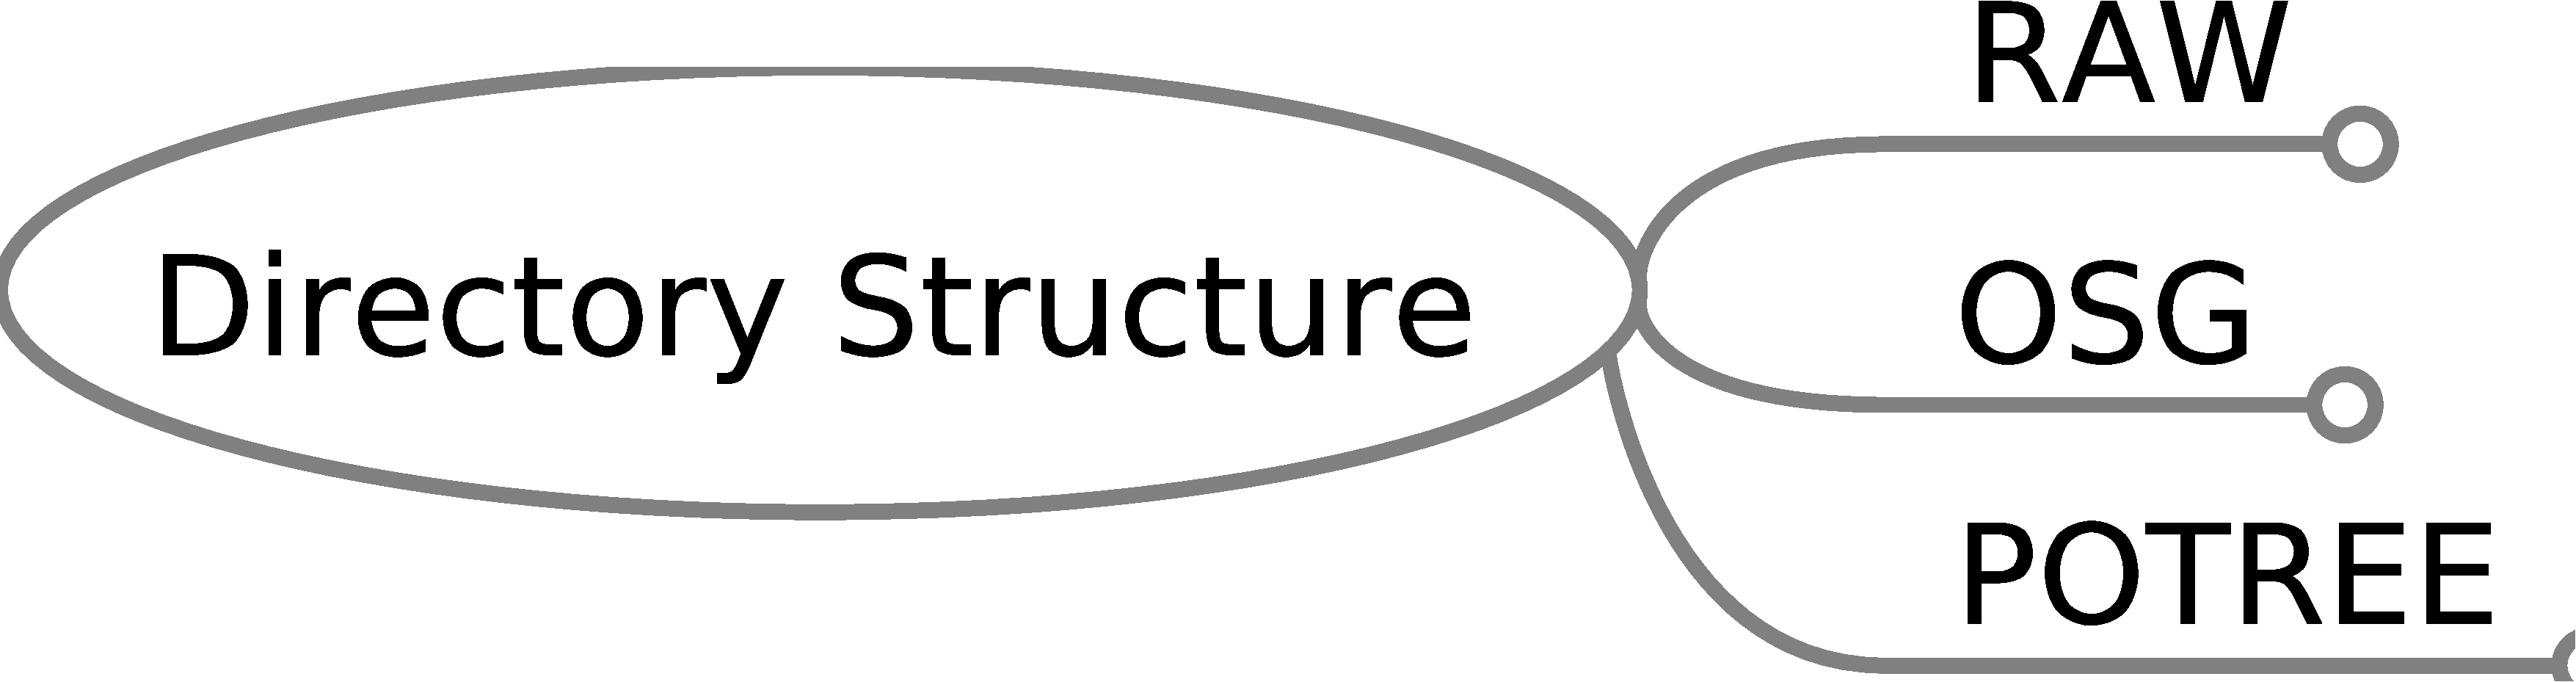
\includegraphics[width=0.4\textwidth]{fig/directory_structure_overview}
 \caption{Overview of the data structure}
 \label{fig:directory_structure_overview}
\end{figure}

\subsubsection{RAW data}
\paragraph{Point clouds}
Higher resolution point clouds are stored in the subdirectories \textit{PC/BACK} and \textit{PC/SITE}, for respectively backgrounds and sites. For backgrounds, the subdirectory contains different folders with point clouds for each background. For sites, the subdirectory contains a separate folder for each site (e.g.\ \textit{PC/SITE/S162} for site 162), which in turn contain different folders for each point cloud of the site. These folders contain LAS files of different point clouds of the site. 

The LAS files contained in each site subfolder may have been pre-aligned (using CloudCompare for example). In that case the LAS file name must be \textbf{*\_ALIGNED\_\textit{BGNAME}*} where \textit{BGNAME} must be the background name (as contained in the folder \textit{PC/BACK/}).
Some point clouds generation tools store the color information in 8 bits instead of the usual 16 bits. In that case the folder name must be \textbf{*\_8BC}. The effect of having an undeclared LAS file with 8 bit color is that the converted data will be black and white. Note that these properties are cumulative, for example \textit{S162\_ALIGNED\_DRIVE\_1\_V3\_8BC} is a valid name for a folder containing a LAS file with 8 bit color information and aligned points.

\begin{figure}[]
 \centering
 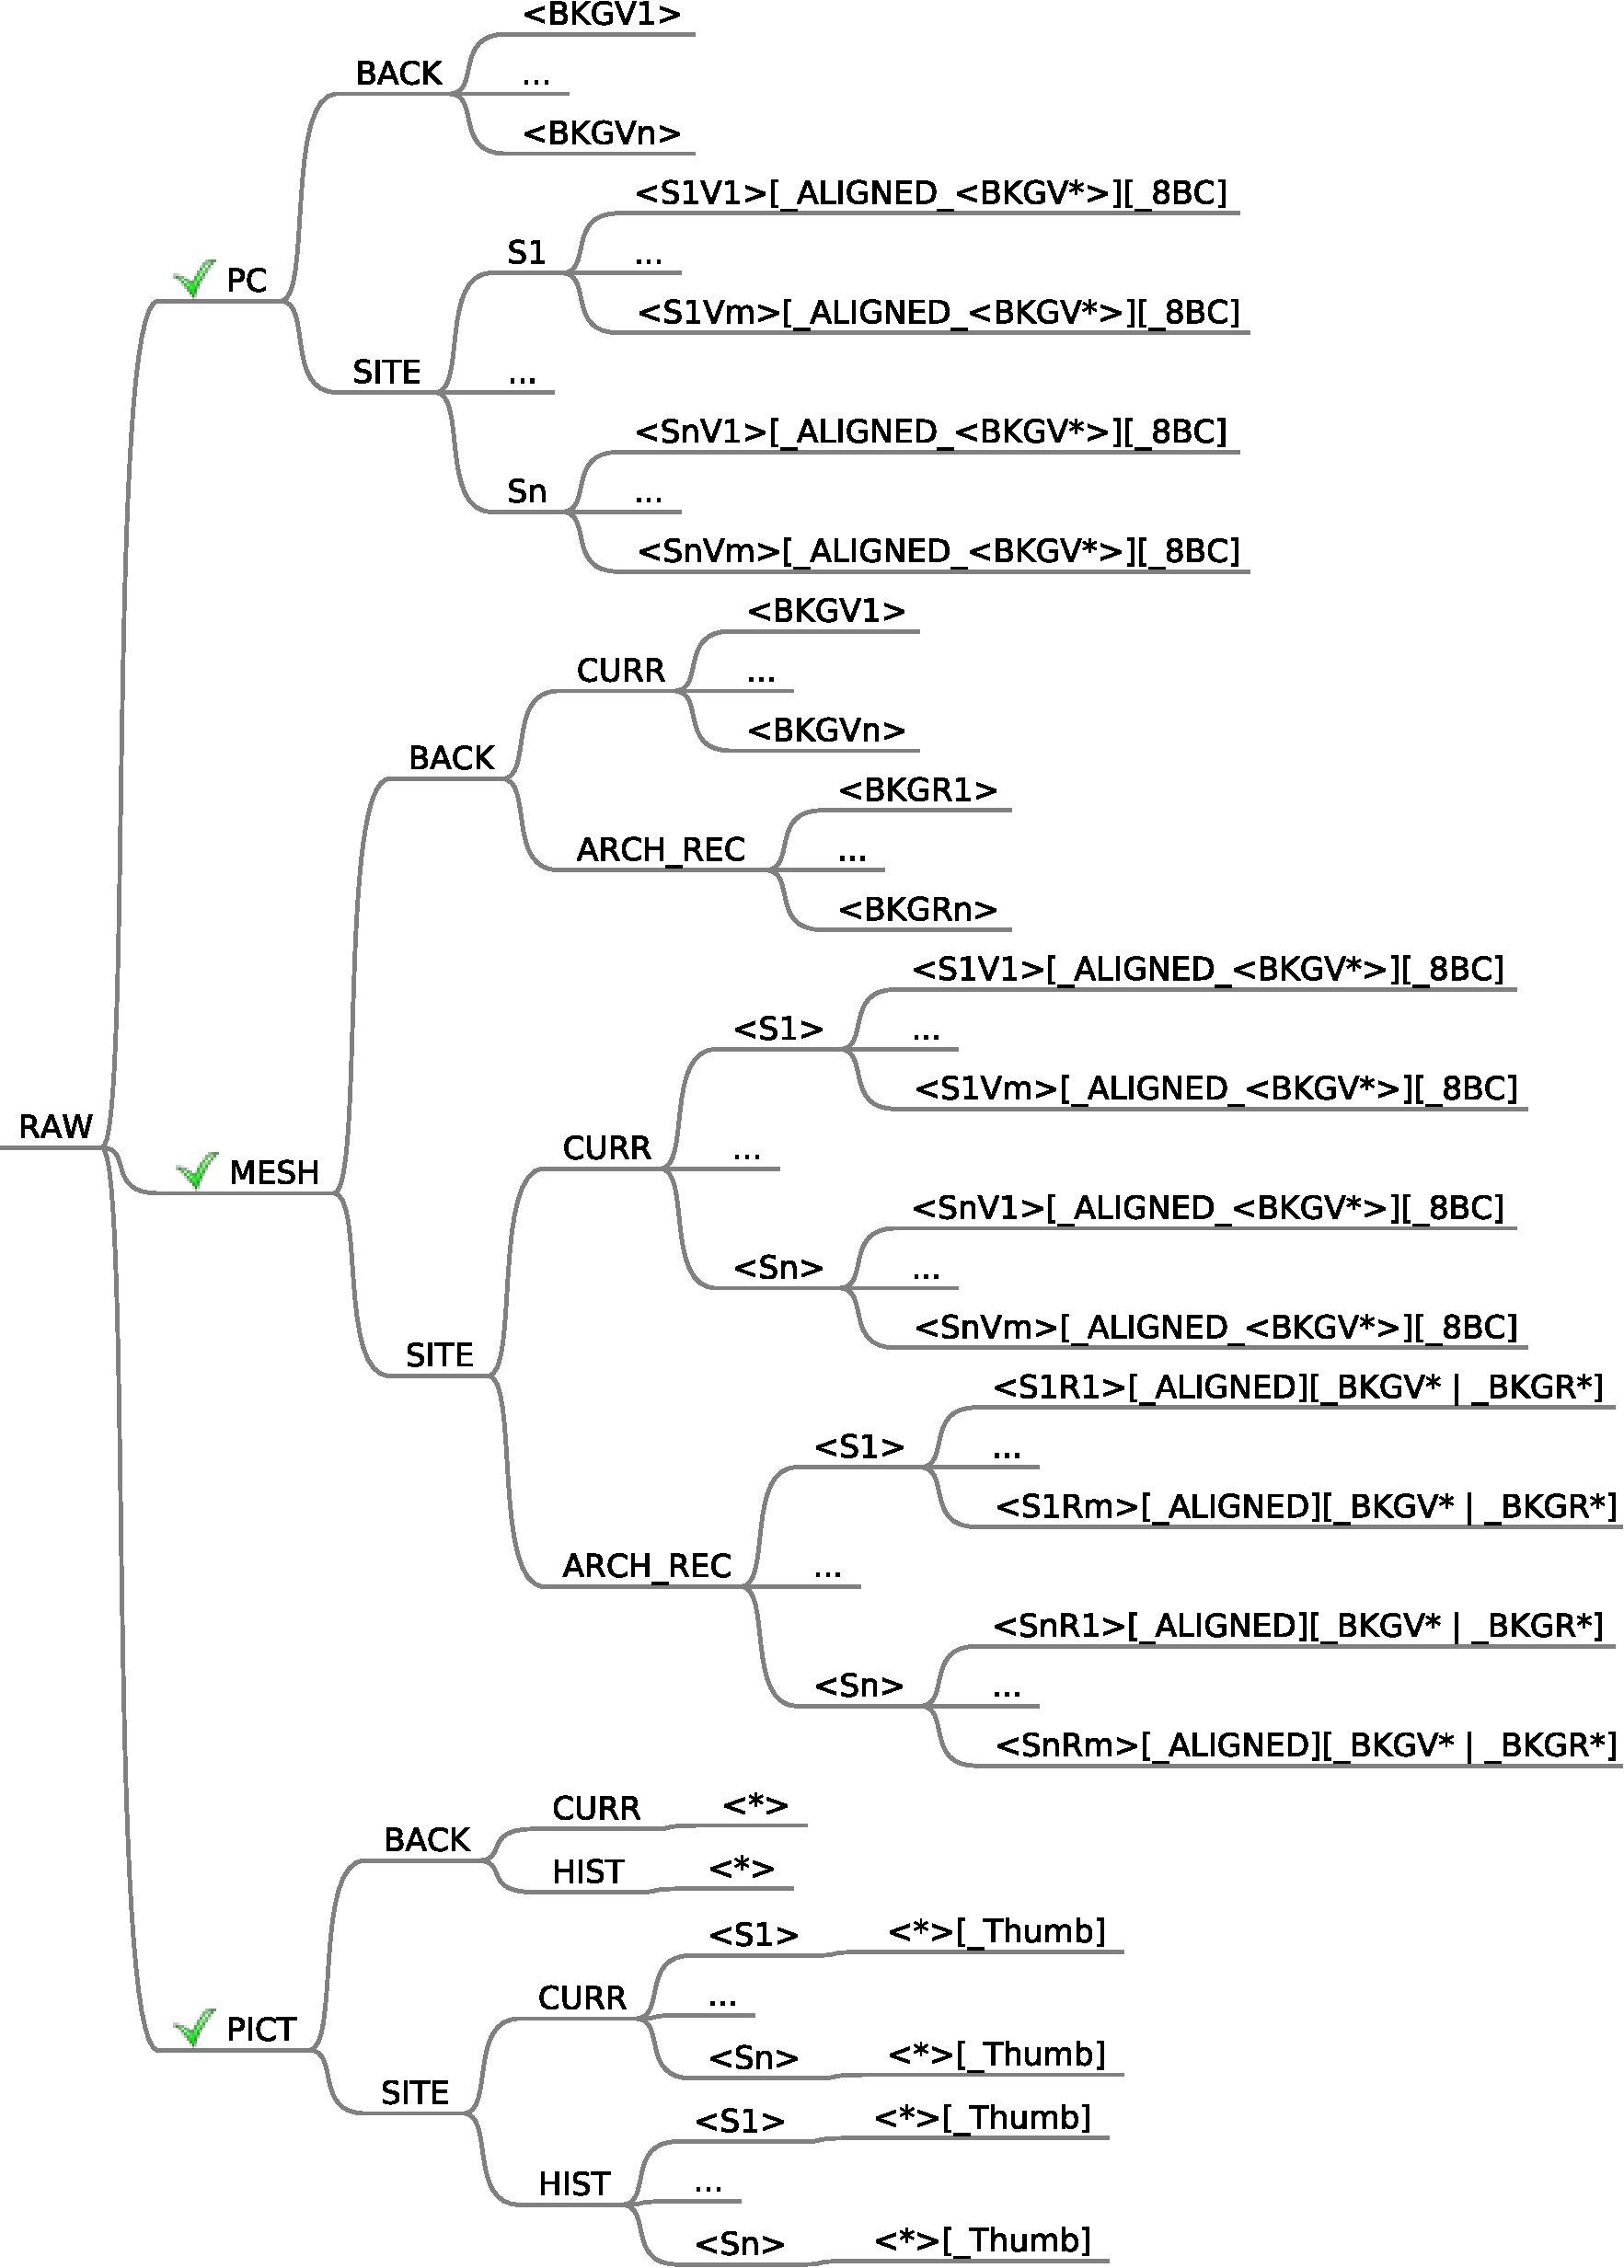
\includegraphics[width=0.8\textwidth]{fig/directory_structure_raw}
 \caption{Overview of the data structure: RAW data items}
 \label{fig:directory_structure_overview_raw}
\end{figure}


\paragraph{Meshes}
Meshes are stored in the directories \textit{MESH/BACK} and \textit{MESH/SITE}, for respectively backgrounds and sites. There are two types of meshes: (a) current  mesh representations, and (b) archeological reconstructions. For backgrounds, they are stored in respectively \textit{MESH/BACK/CURR} and \textit{MESH/BACK/ARCH\_REC}. For sites they are stored in respectively \textit{MESH/SITE/CURR} and \textit{MESH/SITE/ARCH\_REC}. For sites, each of these directories contain different folders for each site. For example the folder \textit{MESH/SITE/CURR/S162} contains mesh representations of the current state of the site 162. 

For each site there must be different folders for the several meshes. Inside these folders the files for the meshes are stored (OBJ, MTL, JPEG). For example \textit{MESH/SITE/CURR/S162} could contain two folders called \textit{162\_curr\_1} and \textit{162\_curr\_2} and each of them contain a OBJ, a MTL and several JPEG files. 

Similarly to the LAS files the meshes can also be aligned. In this case the folder name for a certain mesh must be \textbf{*\_ALIGNED\_\textit{BGNAME}*}. 

\paragraph{Pictures}
Pictures are stored in the subdirectory \textit{PICT}. Pictures can be either of a background or of a site. For both types a further subdivision is made between (a) pictures of the current state of the sites, and (b) historical pictures and paintings. These are stored in respectively \textit{PICT/BACK/CURR} and \textit{PICT/BACK/HIST} for backgrounds, or \textit{PICT/SITE/CURR} and \textit{PICT/SITE/HIST} for sites. For sites, each of these directoryes contains a separate folder for each site. For example the folder \textit{PICT/SITE/CURR/S162} contains pictures of the current state of the site 162.

\subsubsection{OSG data}
The raw data can be converted to the OSGB format. For that purpose a python script \textit{GenerateOSG.py} as been created (section \ref{sec:generatePOTree}). This script should be run with the \textit{vadata} user and should be run when some data has changed in the raw data directory. The POTree data is copied automatically in the POTree data tree, with the naming as specified in figure \ref{fig:directory_structure_overview_osg}.

In order to view the data in your Windows machine you need to download a version of the converted OSG data in your local machine. We use a NLeSC tool called Xenon.

\begin{figure}[!ht]
 \centering
 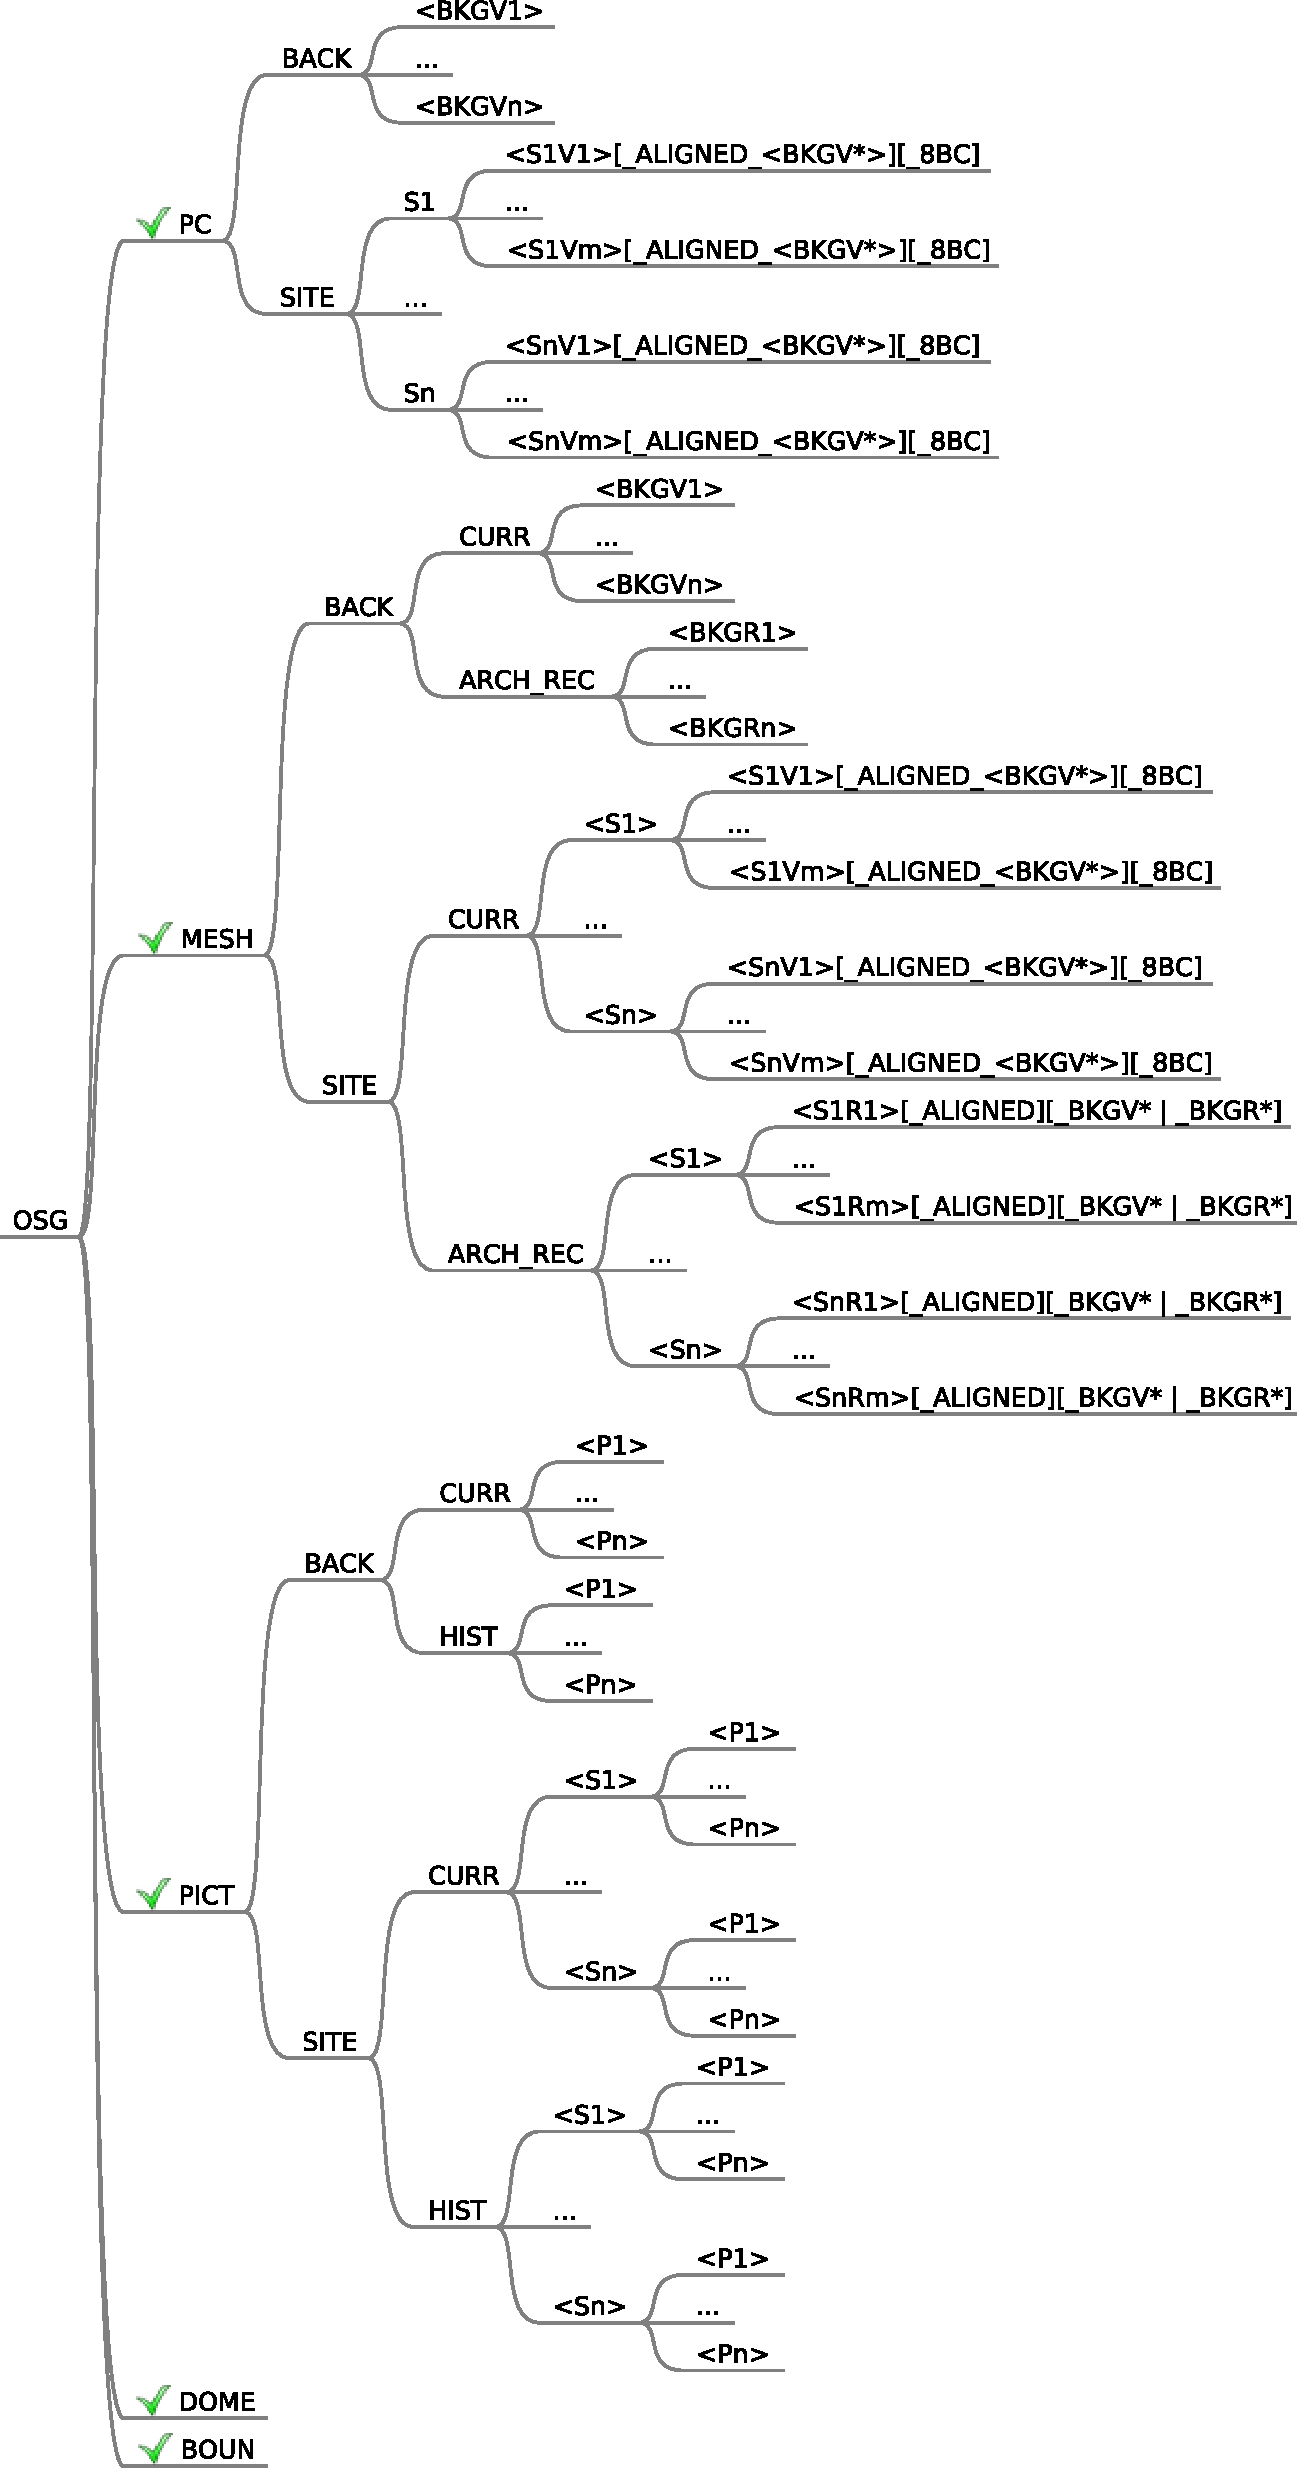
\includegraphics[width=0.75\textwidth]{fig/directory_structure_osg}
 \caption{Overview of the data structure: OSG data items}
 \label{fig:directory_structure_overview_osg}
\end{figure}

\subsubsection{POTree data}
The raw data can be converted to the POTree format. For that purpose a python script \textit{GeneratePOTree.py} has been created (section \ref{sec:generateosg}). This script should be run with the \textit{vadata} user and should be run when some data has changed in the raw data directory. The POTree data is copied automatically in the POTree data tree, with the naming as specified in figure \ref{fig:directory_structure_overview_potree}.

\begin{figure}[!ht]
 \centering
 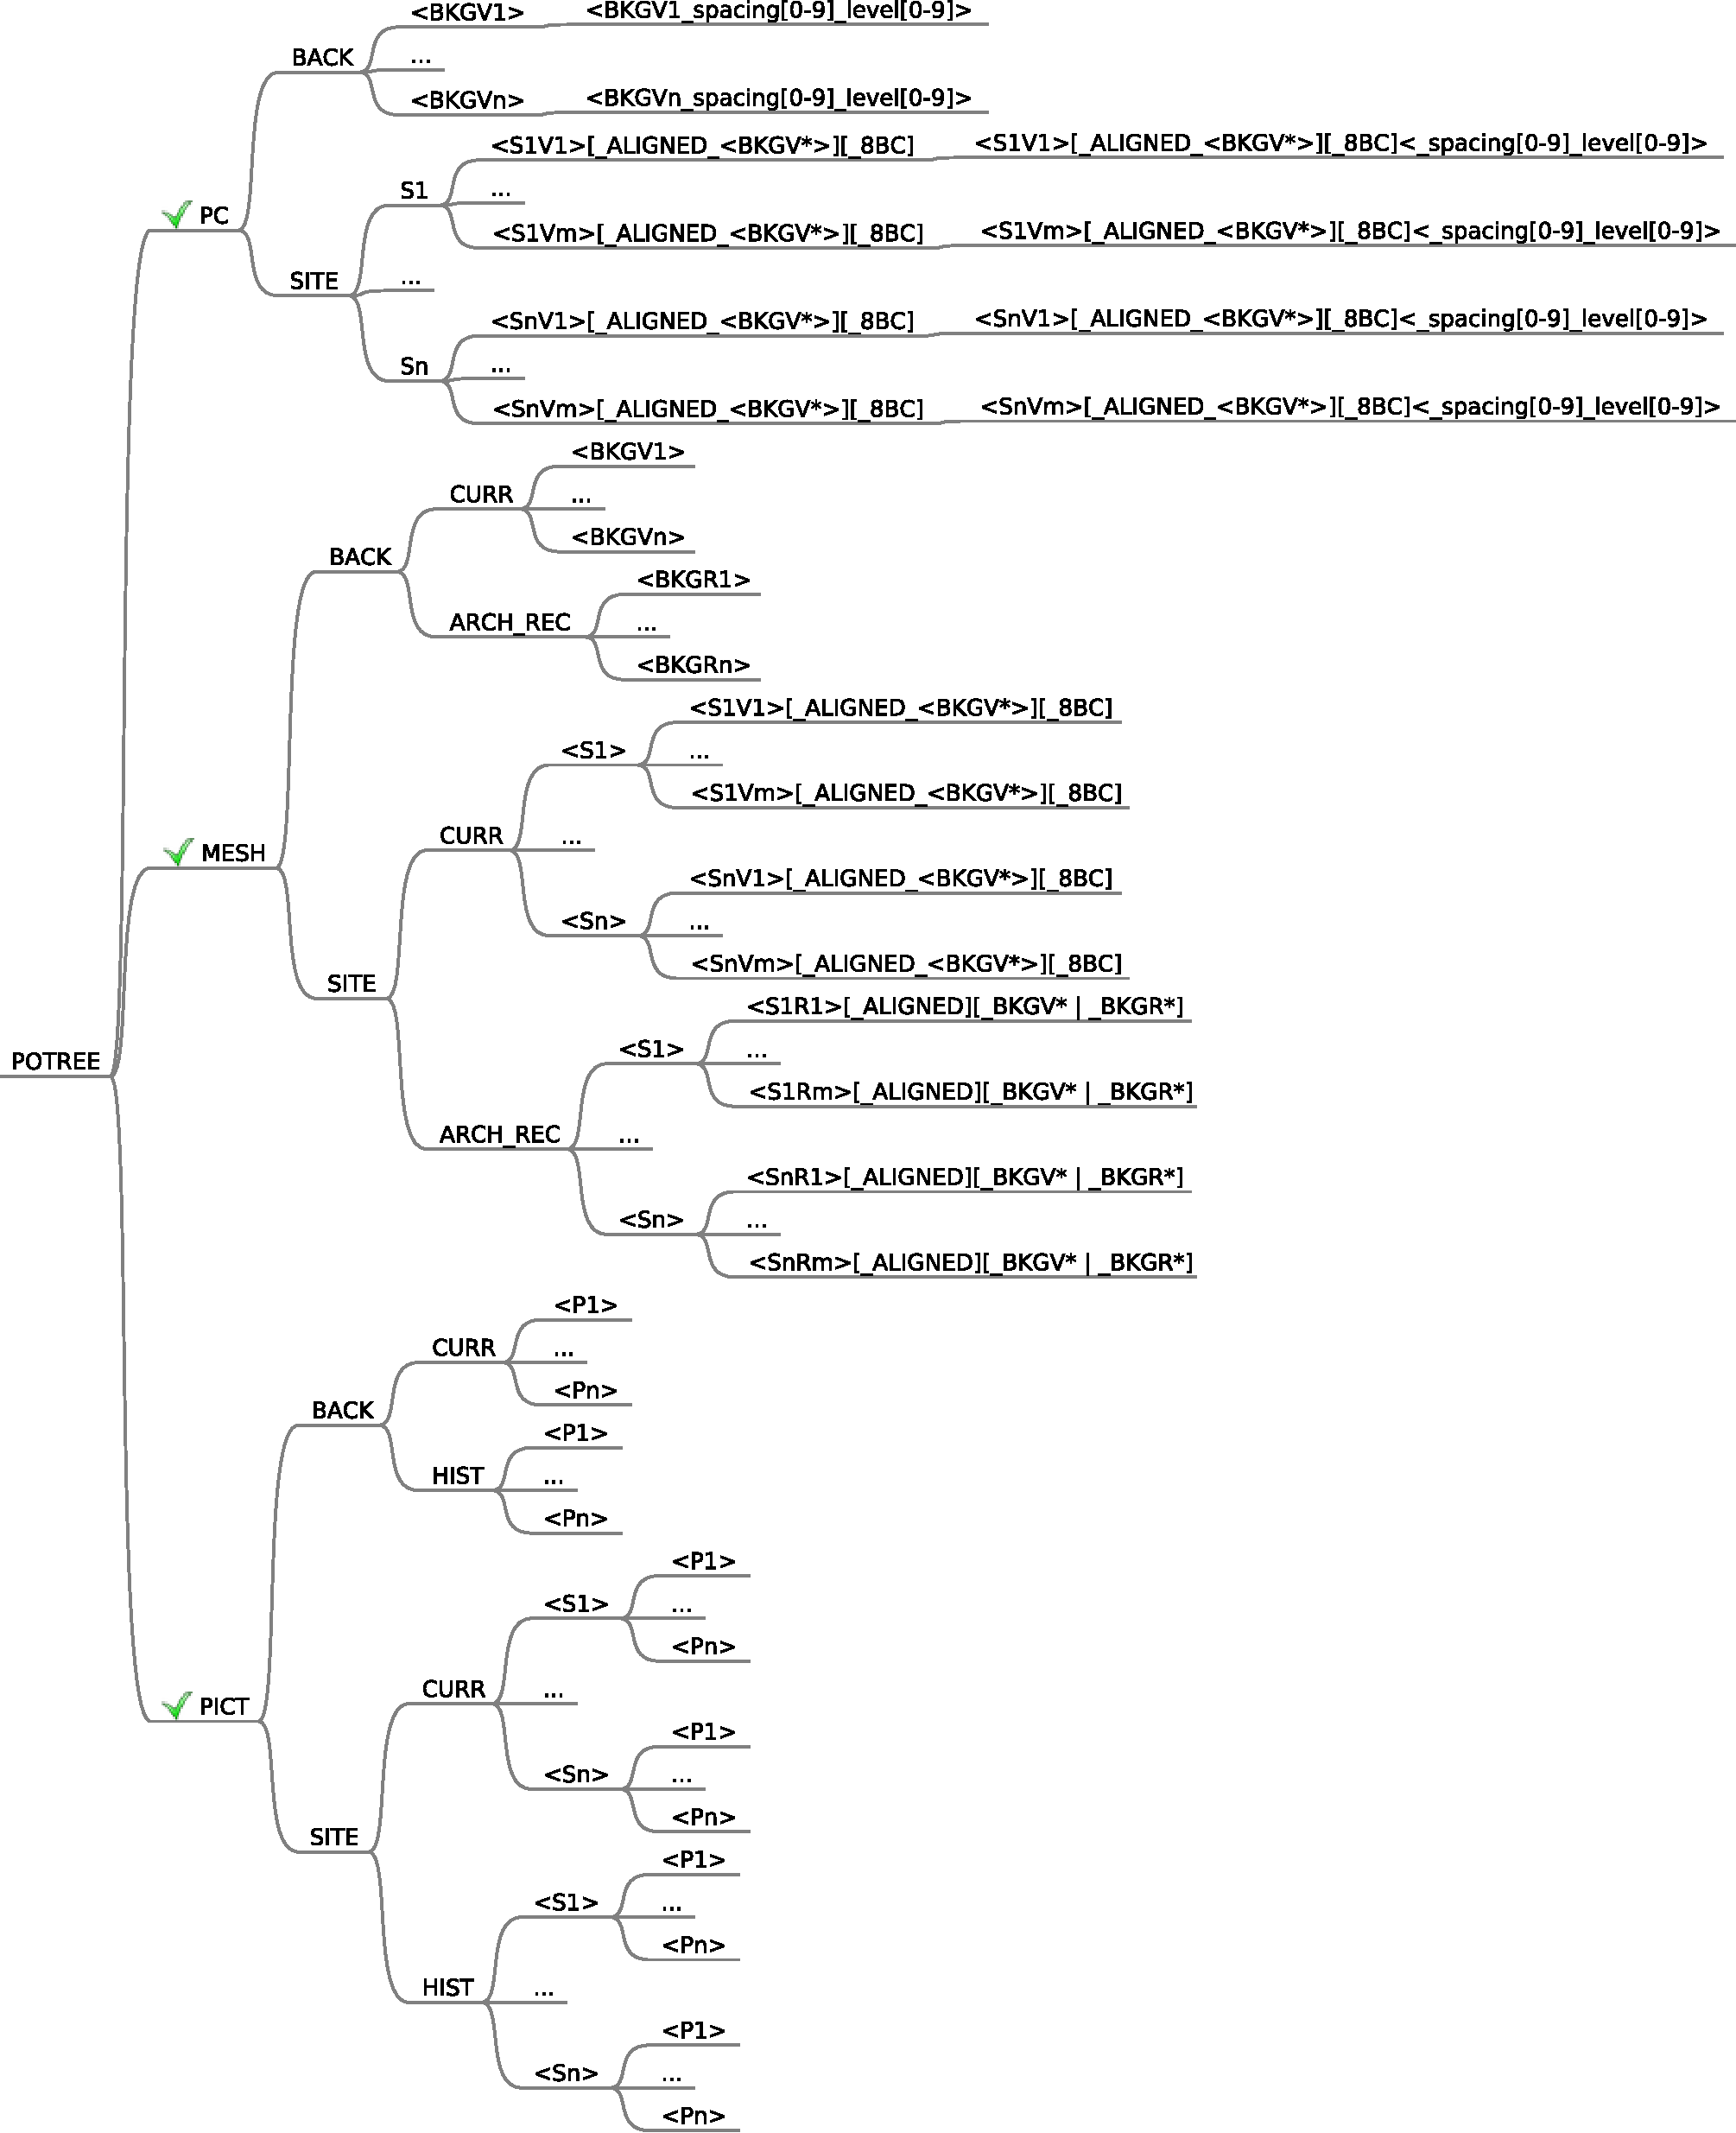
\includegraphics[width=1\textwidth]{fig/directory_structure_potree}
 \caption{Overview of the data structure: POTree data items}
 \label{fig:directory_structure_overview_potree}
\end{figure}


\subsection{Operation on the data structure}
Different operations can be performed on the data structure. The different operations that can be performed are (1) adding RAW data items (section \ref{sec:addraw}); (2) removing RAW data items (section \ref{sec:removeraw}); and (3) listing RAW data items (section \ref{sec:listraw}).

\subsubsection{Adding RAW data items}
\label{sec:addraw}
This section describes the script that should be used to add raw data items to the directory structure: \textit{AddRawDataItem.py}. To run the script, the user needs, depending on the exact datatype, supply additional arguments to the script. An overview of the possible arguments are found in the verbatim below. The script automatically creates a destination folder with the required naming, as specified in section \ref{sec:descriptiondata}, using the supplied arguments.

\begin{Verbatim}[fontfamily=courier,commandchars=\\\{\},fontsize=\footnotesize]
 usage: AddRawDataItem.py [-h] [-i DATA] -k {BACK,SITE} -t {PC,MESH,PICT} -f FILE                                                                                                     
             [-p {CURR,HIST,ARCH_REC}] [-s SRID] [--eight]
             [-l {debug,info,warning,error,critical}] [--site SITE]

Add Raw data item to the file structure.

optional arguments:
  -h, --help            show this help message and exit
  -i DATA, --data DATA  RAW data folder [default /home/pattydat/DATA/RAW]
  -s SRID, --srid SRID  spatial reference system SRID [only for MESH SITE]
  --eight               8 bit color [only for PC SITE or MESH]
  -l {debug,info,warning,error,critical}, --log {debug,info,warning,error,critical}
                        Log level

required arguments:
  -k {BACK,SITE}, --kind {BACK,SITE}
                        Type of item
  -t {PC,MESH,PICT}, --type {PC,MESH,PICT}
                        Type of data
  -f FILE, --file FILE  Input file/directory name to copy

required arguments for MESH and PICT:
  -p {CURR,HIST,ARCH_REC}, --period {CURR,HIST,ARCH_REC}
                        Period (choose from MESH:CURR,ARCH_REC;
                        PICT:CURR,HIST)

required arguments for SITE:
  --site SITE           Site number
\end{Verbatim}

\subsubsection{Removing RAW data items}
\label{sec:removeraw}
This section describes the script that should be used to remove RAW data items from the file structure: \textit{RemoveRawDataItem.py}.
\begin{Verbatim}[fontfamily=courier,commandchars=\\\{\},fontsize=\footnotesize]
usage: RemoveRawDataItem.py [-h] -i ITEMID [-d DBNAME] [-u DBUSER] [-p DBPASS]
                            [-t DBHOST] [-r DBPORT]
                            [-l {debug,info,warning,error,critical}]

Removes a list of Raw data items and their related converted data from the
file structure.

optional arguments:
  -h, --help            show this help message and exit
  -d DBNAME, --dbname DBNAME
                        PostgreSQL DB name vadb]
  -u DBUSER, --dbuser DBUSER
                        DB user [default ronald]
  -p DBPASS, --dbpass DBPASS
                        DB pass
  -t DBHOST, --dbhost DBHOST
                        DB host
  -r DBPORT, --dbport DBPORT
                        DB port
  -l {debug,info,warning,error,critical}, --log {debug,info,warning,error,critical}
                        Log level

required arguments:
  -i ITEMID, --itemid ITEMID
                        Comma-separated list of Raw Data Item Ids Raw data
                        item id (with ? the available raw data items are
                        listed)
\end{Verbatim}

\subsubsection{Listing raw data items}
\label{sec:listraw}
This section describes the script that lists the RAW data items currently in the file structure: \textit{ListRawDataItem.py}.
\begin{Verbatim}[fontfamily=courier,commandchars=\\\{\},fontsize=\footnotesize]
usage: ListRawDataItem.py [-h] [-i ITEMID] [-d DBNAME] [-u DBUSER] [-p DBPASS]
                          [-t DBHOST] [-r DBPORT]
                          [-l {debug,info,warning,error,critical}]

List the Raw data items that are in the DB.

optional arguments:
  -h, --help            show this help message and exit
  -i ITEMID, --itemid ITEMID
                        List the Raw Data Item Ids related to a list of items
                        (comma-separated) [default list all raw data items]
  -d DBNAME, --dbname DBNAME
                        PostgreSQL DB name vadb]
  -u DBUSER, --dbuser DBUSER
                        DB user [default $USERNAME]
  -p DBPASS, --dbpass DBPASS
                        DB pass
  -t DBHOST, --dbhost DBHOST
                        DB host
  -r DBPORT, --dbport DBPORT
                        DB port
  -l {debug,info,warning,error,critical}, --log {debug,info,warning,error,critical}
                        Log level

\end{Verbatim}

\subsubsection{Generating OSG data}
\label{sec:generateosg}
\begin{Verbatim}[fontfamily=courier,commandchars=\\\{\},fontsize=\footnotesize]
 usage: GenerateOSG.py [-h] [-i ITEMID] [-d DBNAME] [-u DBUSER] [-p DBPASS]
                      [-t DBHOST] [-r DBPORT] [-o OSGDIR]
                      [-l {debug,info,warning,error,critical}]

Generates the OSG data for a raw data item.

optional arguments:
  -h, --help            show this help message and exit
  -i ITEMID, --itemid ITEMID
                        Comma-separated list of Raw Data Item Ids [default is
                        to convert all raw data items related to sites that do
                        not have a related OSG data item] (with ? the
                        available raw data items are listed, with ! the list
                        all the raw data items without any related OSG data
                        item)
  -d DBNAME, --dbname DBNAME
                        Postgres DB name [default vadb]
  -u DBUSER, --dbuser DBUSER
                        DB user [default $USERNAME]
  -p DBPASS, --dbpass DBPASS
                        DB pass
  -t DBHOST, --dbhost DBHOST
                        DB host
  -r DBPORT, --dbport DBPORT
                        DB port
  -o OSGDIR, --osgDir OSGDIR
                        OSG data directory [default /home/pattydat/DATA/OSG]
  -l {debug,info,warning,error,critical}, --log {debug,info,warning,error,critical}
                        Log level
\end{Verbatim}

\subsubsection{Generating POTree data}
\label{sec:generatePOTree}
\begin{Verbatim}[fontfamily=courier,commandchars=\\\{\},fontsize=\footnotesize]
usage: GeneratePOTree.py [-h] [-i ITEMID] [-d DBNAME] [-u DBUSER] [-p DBPASS]
                         [-t DBHOST] [-r DBPORT] [-o POTREEDIR]
                         [--levels LEVELS]
                         [-l {debug,info,warning,error,critical}]

Generates the POTree data for a raw data item (ONLY FOR PCs)

optional arguments:
  -h, --help            show this help message and exit
  -i ITEMID, --itemid ITEMID
                        Comma-separated list of PointCloud Raw Data Item Ids
                        [default is to convert all raw data items that do not
                        have a related POtree data item] (with ? the available
                        raw data items are listed, with ! the list all the raw
                        data items without any related POTree data item)
  -d DBNAME, --dbname DBNAME
                        Postgres DB name [default vadb]
  -u DBUSER, --dbuser DBUSER
                        DB user [default ronald]
  -p DBPASS, --dbpass DBPASS
                        DB pass
  -t DBHOST, --dbhost DBHOST
                        DB host
  -r DBPORT, --dbport DBPORT
                        DB port
  -o POTREEDIR, --potreeDir POTREEDIR
                        POTREE data directory [default
                        /home/pattydat/DATA/POTREE]
  --levels LEVELS       Number of levels of the Octree, parameter for
                        PotreeConverter. [default is 4 for Sites and 8 for
                        Backgrounds]
  -l {debug,info,warning,error,critical}, --log {debug,info,warning,error,critical}
                        Log level
\end{Verbatim}
